\chapter{Fermi Polaron}
\label{chapter:fermi-polaron}

In this Chapter, we consider the extremely spin-imbalanced case in which there is only one spin-$\downarrow$ impurity inside a Fermi sea of spin-$\uparrow$ particles. This scenario is well-known as the Fermi polaron problem and has been studied extensively in vacuum~\cite{Schmidt2011,Kamikado2017}. However, spectral properties at finite temperature were just recently investigated by Hu et al.~\cite{Hu2022} with a non-selfconsistent approach. In the following, we apply our fully selfconsistent real-time framework to study the spectral and quasiparticle properties of the Fermi polaron at finite temperature.

\section{Theoretical description}
\label{section:polaron-theoretical-description}

In this Section, we introduce the general theoretical description of a single impurity immersed in a Fermi sea of particles with different spin and derive the selfconsistent equations. The general microscopic action which accounts for spin and mass imbalance is given by
%
\begin{align}
	\label{eq:polaron-action}
    S[\psi, \phi] = \int_{\tau,\bm{x}}\,
    \Big[ \sum_{\sigma=\uparrow,\downarrow} \psi^*_{\sigma} (\partial_{\tau} - \nabla^2/(2m_{\sigma}) - \mu_{\sigma}) \psi_{\sigma}
    + \nu \phi^* \phi - h (\phi^* \psi_{\uparrow} \psi_{\downarrow} - \phi \psi^*_{\uparrow} \psi^*_{\downarrow}) \Big] \,,
\end{align}
%
where $2m_{\uparrow} = 1$ and $\mu_{\uparrow}$ is the mass and chemical potential of the majority atoms, and $2m_{\downarrow} = (1+\alpha)/(1-\alpha)$ and $\mu_{\downarrow}\leq 0$ is for the impurity. The mass imbalance $\alpha$ is connected to the reduced mass $2m_r = (1+\alpha)/2$ and satisfies $-1 < \alpha = (m_{\downarrow}-m_{\uparrow})/(m_{\downarrow}+m_{\uparrow}) < 1$.

The selfconsistent equations for the Fermi polaron problem can be derived by the same means as described in Chapter~\ref{chapter:bcs-bec-crossover}, however, some simplifications can be made. First of all, we can replace again all three-point functions by the classical vertices $\Gamma^{(3)}=S^{(3)}$. Moreover, since there is only one impurity in the system, the majority atoms are barely affected and can be treated as non-interacting particles. The simplified Dyson-Schwinger equations for the Fermi polaron problem are shown diagrammatically in Fig.~\ref{fig:polaron_DSEs} and will be discussed in the following. It is well-known that the strong spin-imbalance hinders the system to form a condensate, such that the physics is described completely by the normal phase~\cite{Punk2010}. However, there is still a non-trivial polaron-to-molecule phase transition~\cite{Schmidt2013}.

As pointed out before, the spin-$\uparrow$ majority atoms in the Fermi sea are not dressed and can be described by the classical fermion Green's function
%
\begin{align}
	\label{eq:maj}
    G^{(0)}_{\uparrow}(\omega_n, \bm{p})
    = \frac{1}{-i\omega_n+\varepsilon_{\bm{p}}-\mu_{\uparrow}} \,.
\end{align}
%
where $\varepsilon_{\bm{p}}=\bm{p}^2/(2m_{\uparrow})=\bm{p}^2$ is the majority dispersion relation. However, the impurity Green's function obtains a self-energy and can be written as (see Eq.~\eqref{eq:selfconsistent-equations})
%
\begin{align}
	\label{eq:min}
    G_{\downarrow}(\omega_n, \bm{p})
    = \frac{1}{-i\omega_n+\varepsilon^{(I)}_{\bm{p}}-\mu_{\downarrow}
    -\Sigma(\omega_n, \bm{p})} \,,
\end{align}
%
where $\varepsilon^{(I)}_{\bm{p}}=\bm{p}^2/(2m_{\downarrow}) = \bm{p}^2\,(1-\alpha)/(1+\alpha)$ is the impurity dispersion relation~\cite{Hu2022}.

\begin{figure}[t]
	\begin{center}
		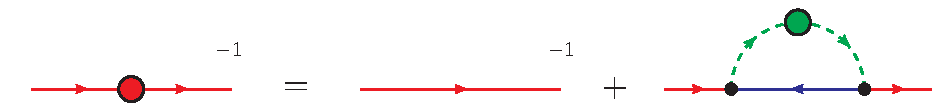
\includegraphics[width=0.8\textwidth]{figs/polaron_prop_DSE.pdf} \\
		\vspace{0.5cm}
		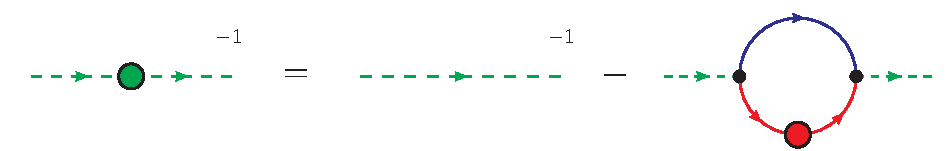
\includegraphics[width=0.8\textwidth]{figs/polaron_boson_DSE.pdf} 
	\end{center}
	\caption[Polaron Dyson-Schwinger equations]{Simplified Dyson-Schwinger equations for the Fermi polaron. The blue propagator of the Fermi sea is just the classical fermion propagator and only the red polaron Greens function gets dressed. All vertices are classical.}
	\label{fig:polaron_DSEs}
\end{figure}

The impurity self-energy $\Sigma(\omega_n, \bm{p})$ is given by (see Fig.~\ref{fig:polaron_DSEs})
%
\begin{align}
	\label{eq:self}
    \Sigma(\omega_n, \bm{p})
    = h^2 \int\frac{d^{3}q}{(2\pi)^{3}}\, T\sum_{\Omega_m}
    G_{\phi}(\Omega_m, \bm{q})
    G^{(0)}_{\uparrow}(\Omega_m-\omega_n, \bm{q-p}) \,.
\end{align}
%
And the molecule propagator $G_{\phi}(\omega_m, \bm{q})$ satisfies again the relation~\eqref{eq:selfconsistent-equations}
%
\begin{align}
	\label{eq:mol}
    G^{-1}_{\phi}(\omega_m, \bm{q}) = -\frac{h^2}{8\pi a} - \Pi(\omega_n,\bm{p}) \,,
\end{align}
%
with the molecule self-energy $\Pi(\omega_n,\bm{p})$ given by
%
\begin{align}
	\label{eq:pol}
    \Pi(\omega_n, \bm{p}) =
    h^2 \int\frac{d^{3}q}{(2\pi)^{3}}\left[ T\sum_{\Omega_m} G_{\downarrow}(\Omega_m, \bm{q}) G^{(0)}_{\uparrow}(\omega_n-\Omega_m, \bm{p-q}) - \frac{1+\alpha}{2\bm{q}^2} \right] \,,
\end{align}
%
where the counterterm changed because of the mass-imbalance~\cite{Hu2022}.

Again, these coupled equations can be solved selfconsistently in real frequencies with the spectral representation. Analytical continuation $i\omega_n = \omega + i0^+$ to the retarded self-energies and taking the imaginary part yields (see Eq.~\eqref{eq:imaginary-part-self-energies})
%
\begin{align}
	\label{eq:imaginary-part-polaron-self-energies}
	\mathrm{Im}\,\Sigma^R(\omega,\bm{p}) &= -\pi h^2\int_{\bm{q}}
	\rho_{\phi}(\omega+\varepsilon_{\bm{q-p}}-\mu_{\uparrow},\bm{q})
	\,n_F(\varepsilon_{\bm{q-p}}-\mu_{\uparrow}) \,, \notag \\
	\mathrm{Im}\,\Pi^R(\omega,\bm{p}) &= \pi h^2\int_{\bm{q}}
	\rho_{\downarrow}(\omega-\varepsilon_{\bm{p-q}}+\mu_{\uparrow},\bm{q})
	\left[1-n_F(\varepsilon_{\bm{p-q}}-\mu_{\uparrow})\right] \,.
\end{align}
%
Here, we used the fact that the quantum statistics of the impurity is not relevant and the molecule occupation number is vanishingly small in the single-impurity limit~\cite{Hu2022}. For a finite impurity concentration, one has to be a bit more careful, see~\cite{Hu2018,Tajima2019}. Additionally, we are left with only 2-dimensional integrals since the majority is non-interacting and the spectral parameter can be integrated out.

From here, the real part can be obtained again via the Kramers-Kronig relation~\eqref{eq:kramers-kronig} and all the numerical steps stay the same. For the boson self-energy, the same subtraction schemes can be used. We refer the reader to Appendix~\ref{app:boson-self-energy-calculation} and~\ref{app:numerical-implementation} for more details on the analytical results and numerical implementation.


\section{Results}
\label{section:polaron-results}

The Fermi polaron problem has been studied intensively in previous works. First excitation spectra at zero temperature were obtained by R. Schmidt and T. Enss using fRG and Padé approximation methods in~\cite{Schmidt2011}. Their results were confirmed and generalized with the fRG in real frequencies by K. Kamikado et al. in~\cite{Kamikado2017}. Since then a numerous amount of articles concerning the quasiparticle properties of the 3-dimensional Fermi polaron have been published~\cite{Mulkerin2019,Scazza2022,Veillette2008,Vlietinck2013}. Also spin-imbalanced gases in general have been investigated with different methods~\cite{Chevy2006,Prokofev2008,VanHoucke2020,Veillette2008}. Recently, also 2-dimensional Fermi gases~\cite{Schmidt2012,Bauer2014,Mulkerin2015}, Bose polarons~\cite{Tajima2021} and general Bose-Fermi mixtures~\cite{Milczewski2022} have been studied.

With the spectral approach described above, we can obtain spectral functions at arbitrary temperatures and mass-imbalances. In this part, we will show the equivalence to previous works for the mass-balanced case and discuss possible generalizations. In the end, selfconsistent and non-selfconsistent results for the rf spectra of the unitary Fermi polaron are presented and compared to recent works~\cite{Tajima2019,Hu2008,Yan2019}. 

Let us begin with a general discussion of the results at zero temperature. These are obtained by replacing $n_F(x)\rightarrow\theta(-x)$, as mentioned in Section~\ref{section:normal-phase}, and using the vacuum boson self-energy. Fig.~\ref{fig:specs-comparison} shows the selfconsistent polaron spectral functions at $T=0$ for different interaction strengths. These results agree well with the ones obtained in~\cite{Schmidt2011,Kamikado2017} using the fRG. For the polaron ground state energy at unitarity, we obtain $\mu_{\downarrow}\simeq-0.62$ which compares favorably with~\cite{Combescot2008}. The non-selfconsistent result is $\mu_{\downarrow}\simeq-0.61$ and shows the equivalence to Chevy's variational  ansatz~\cite{Chevy2006,Combescot2007}. In vacuum, the chemical potential of the non-interacting Fermi sea is $\mu_{\uparrow}=1$. Contrary to the spin-balanced case, the Padé approximation method from~\cite{Schmidt2011} is quite reasonable in the polaron case. This might stem from the fact that the majority particles are not dressed and the structure of the polaron spectral function is simpler. However, only real-time approaches, like in~\cite{Kamikado2017} or this work, can compute fully correct spectral functions.

\begin{figure}[b]
	\centering
	\subfigure[$(k_Fa)^{-1} = -0.5$]{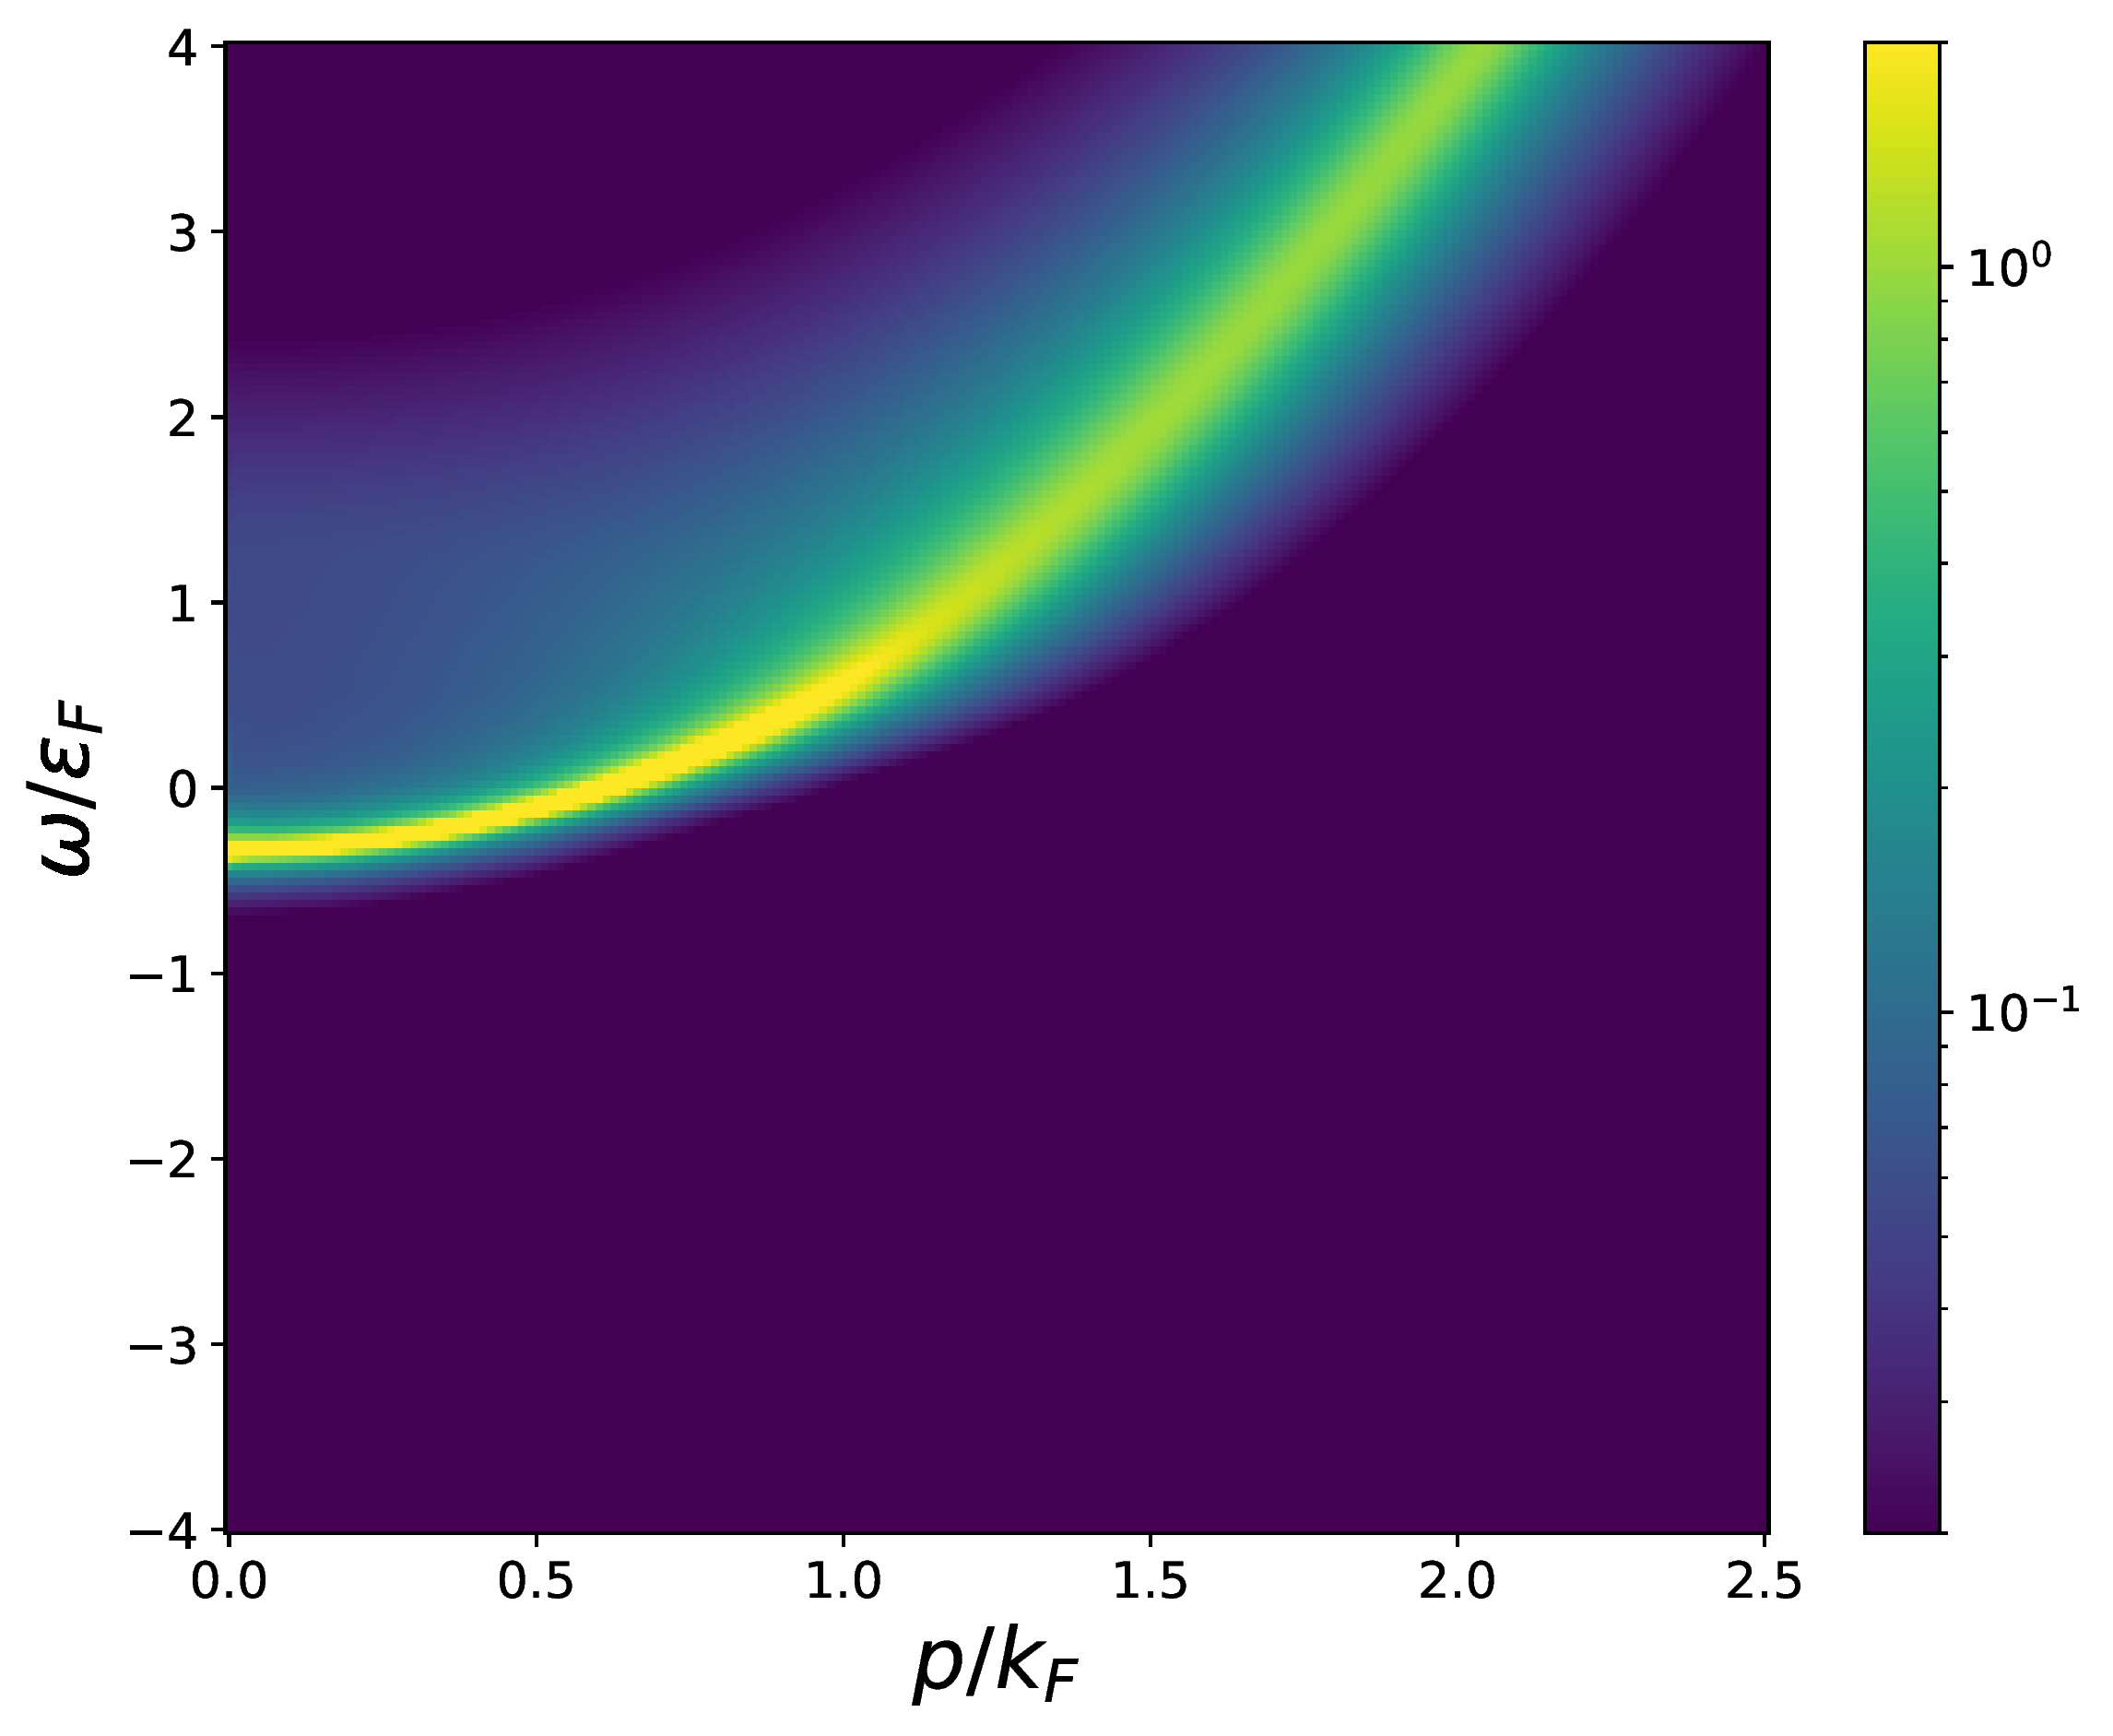
\includegraphics[width=0.24\textwidth]{figs/polaron_n05kfa.png}} 
	\subfigure[$(k_Fa)^{-1} = 0$]{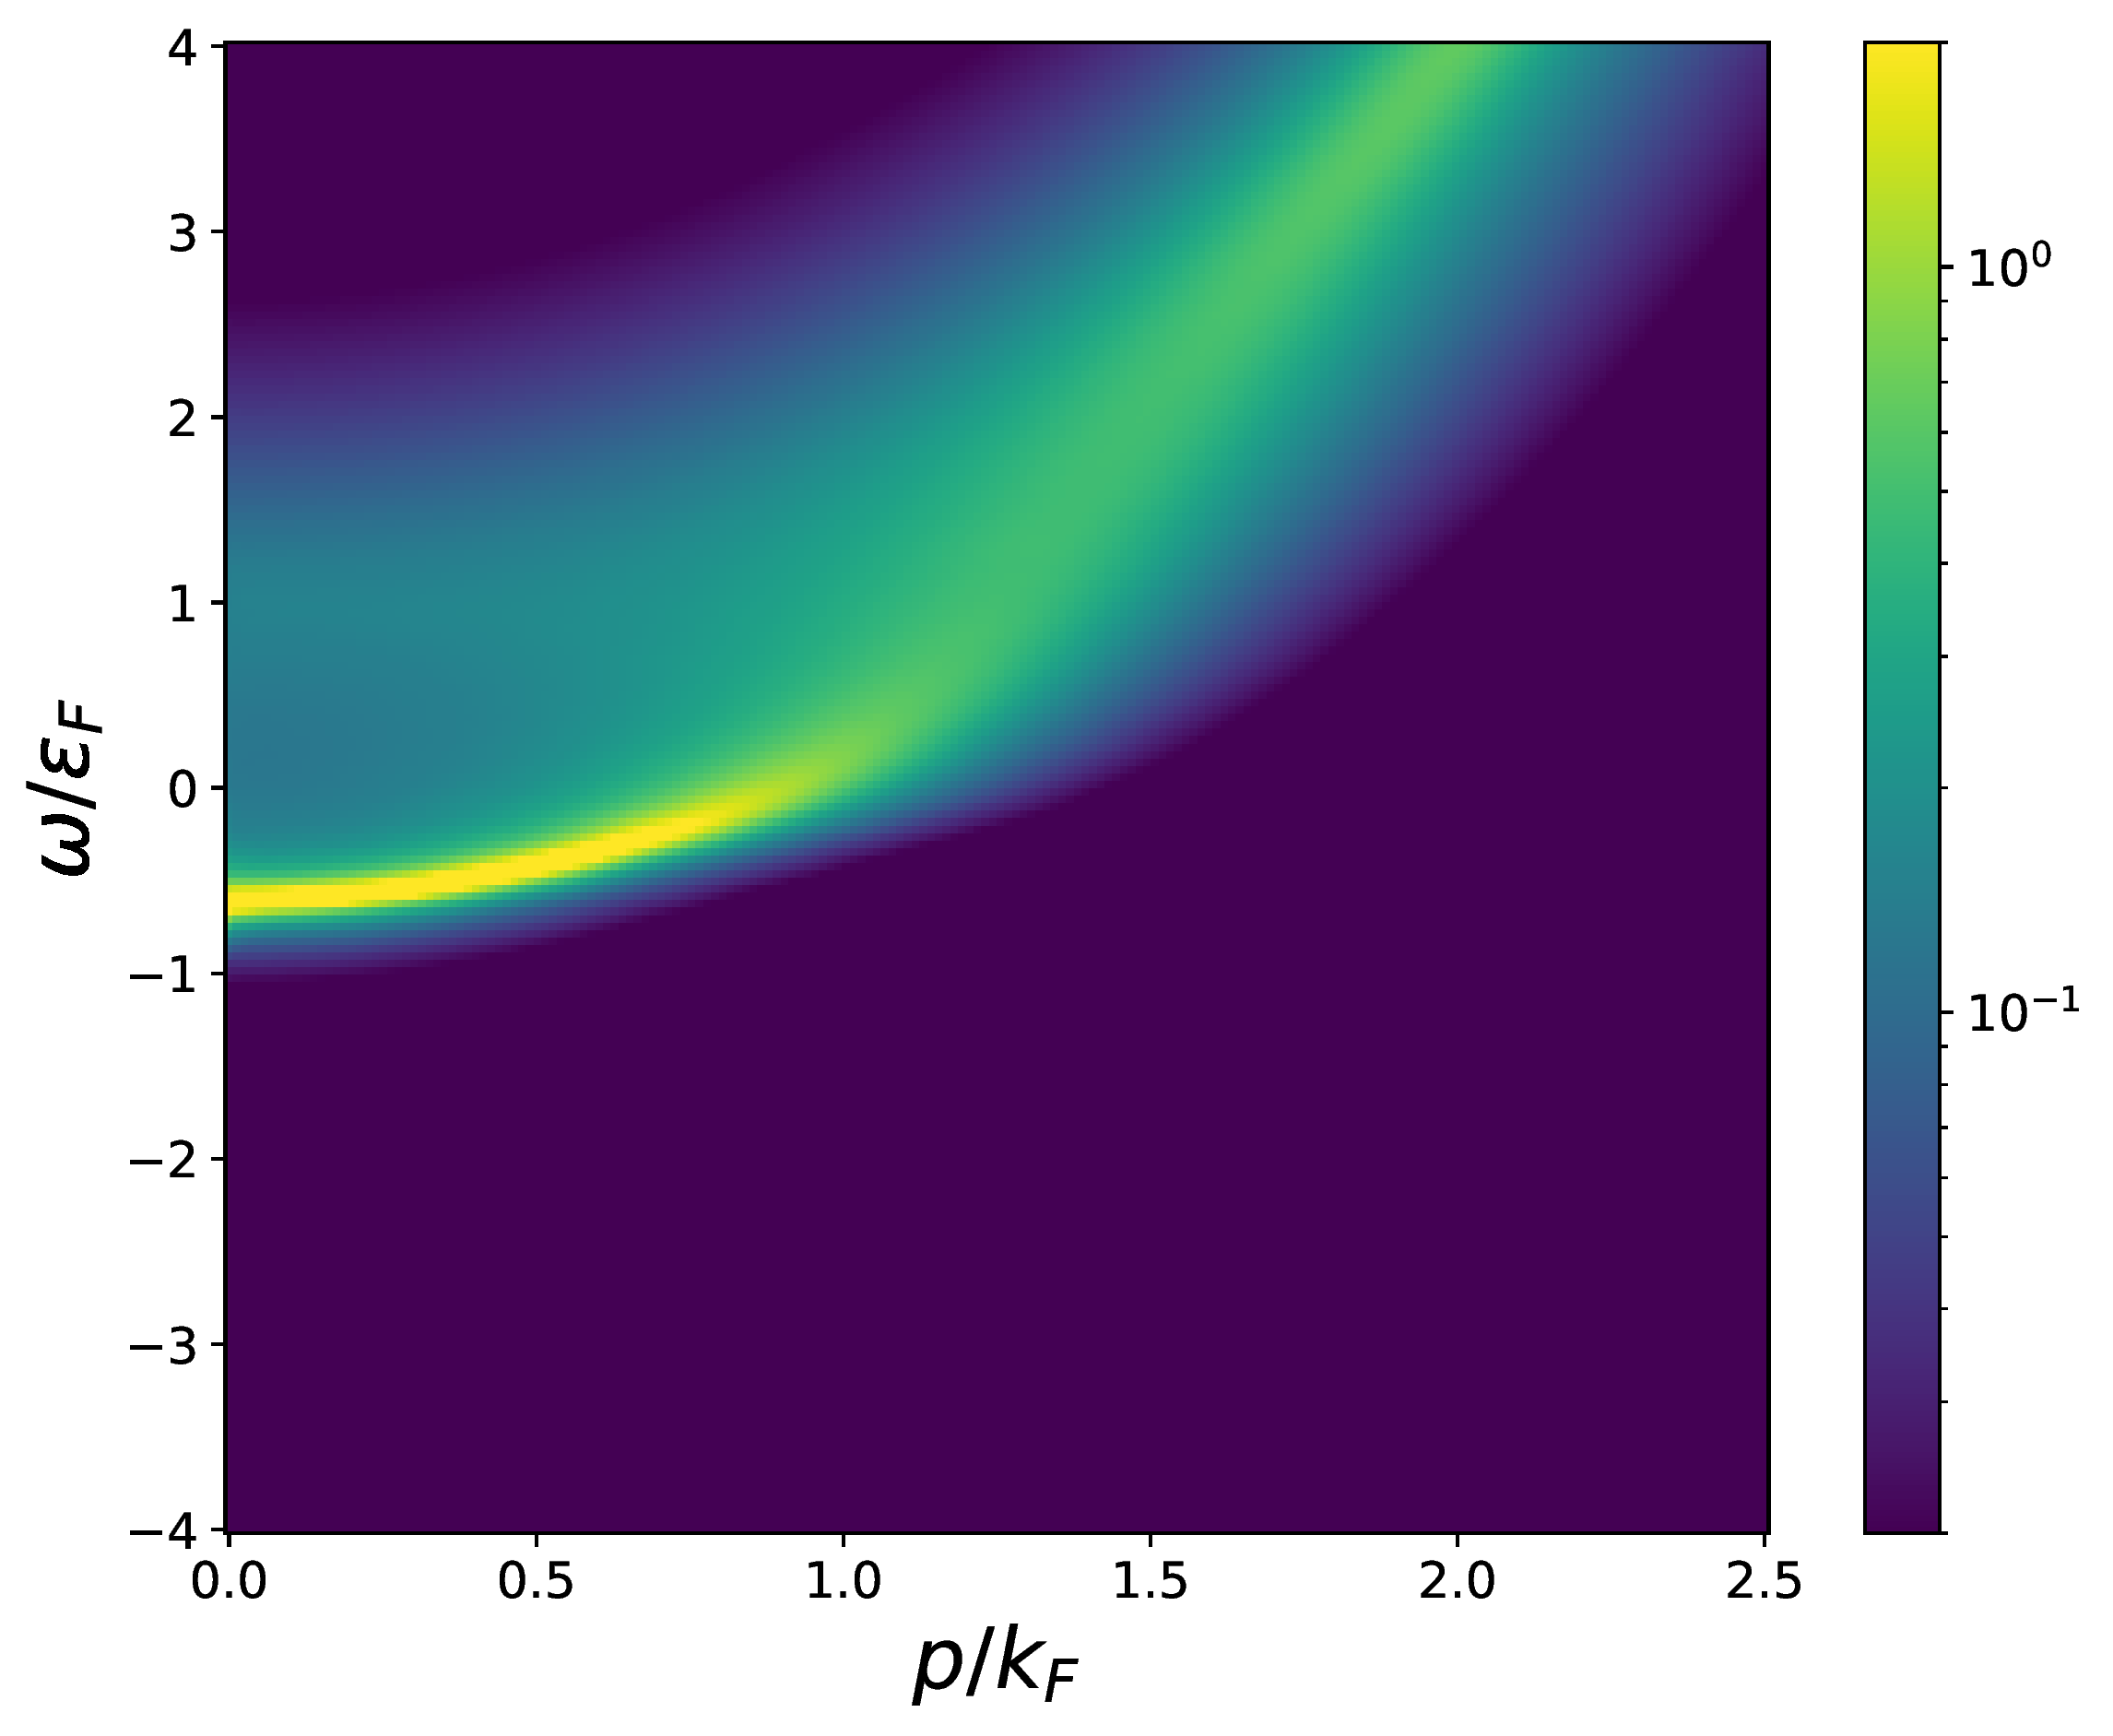
\includegraphics[width=0.24\textwidth]{figs/polaron_unitary0.png}} 
	\subfigure[$(k_Fa)^{-1} = 0.5$]{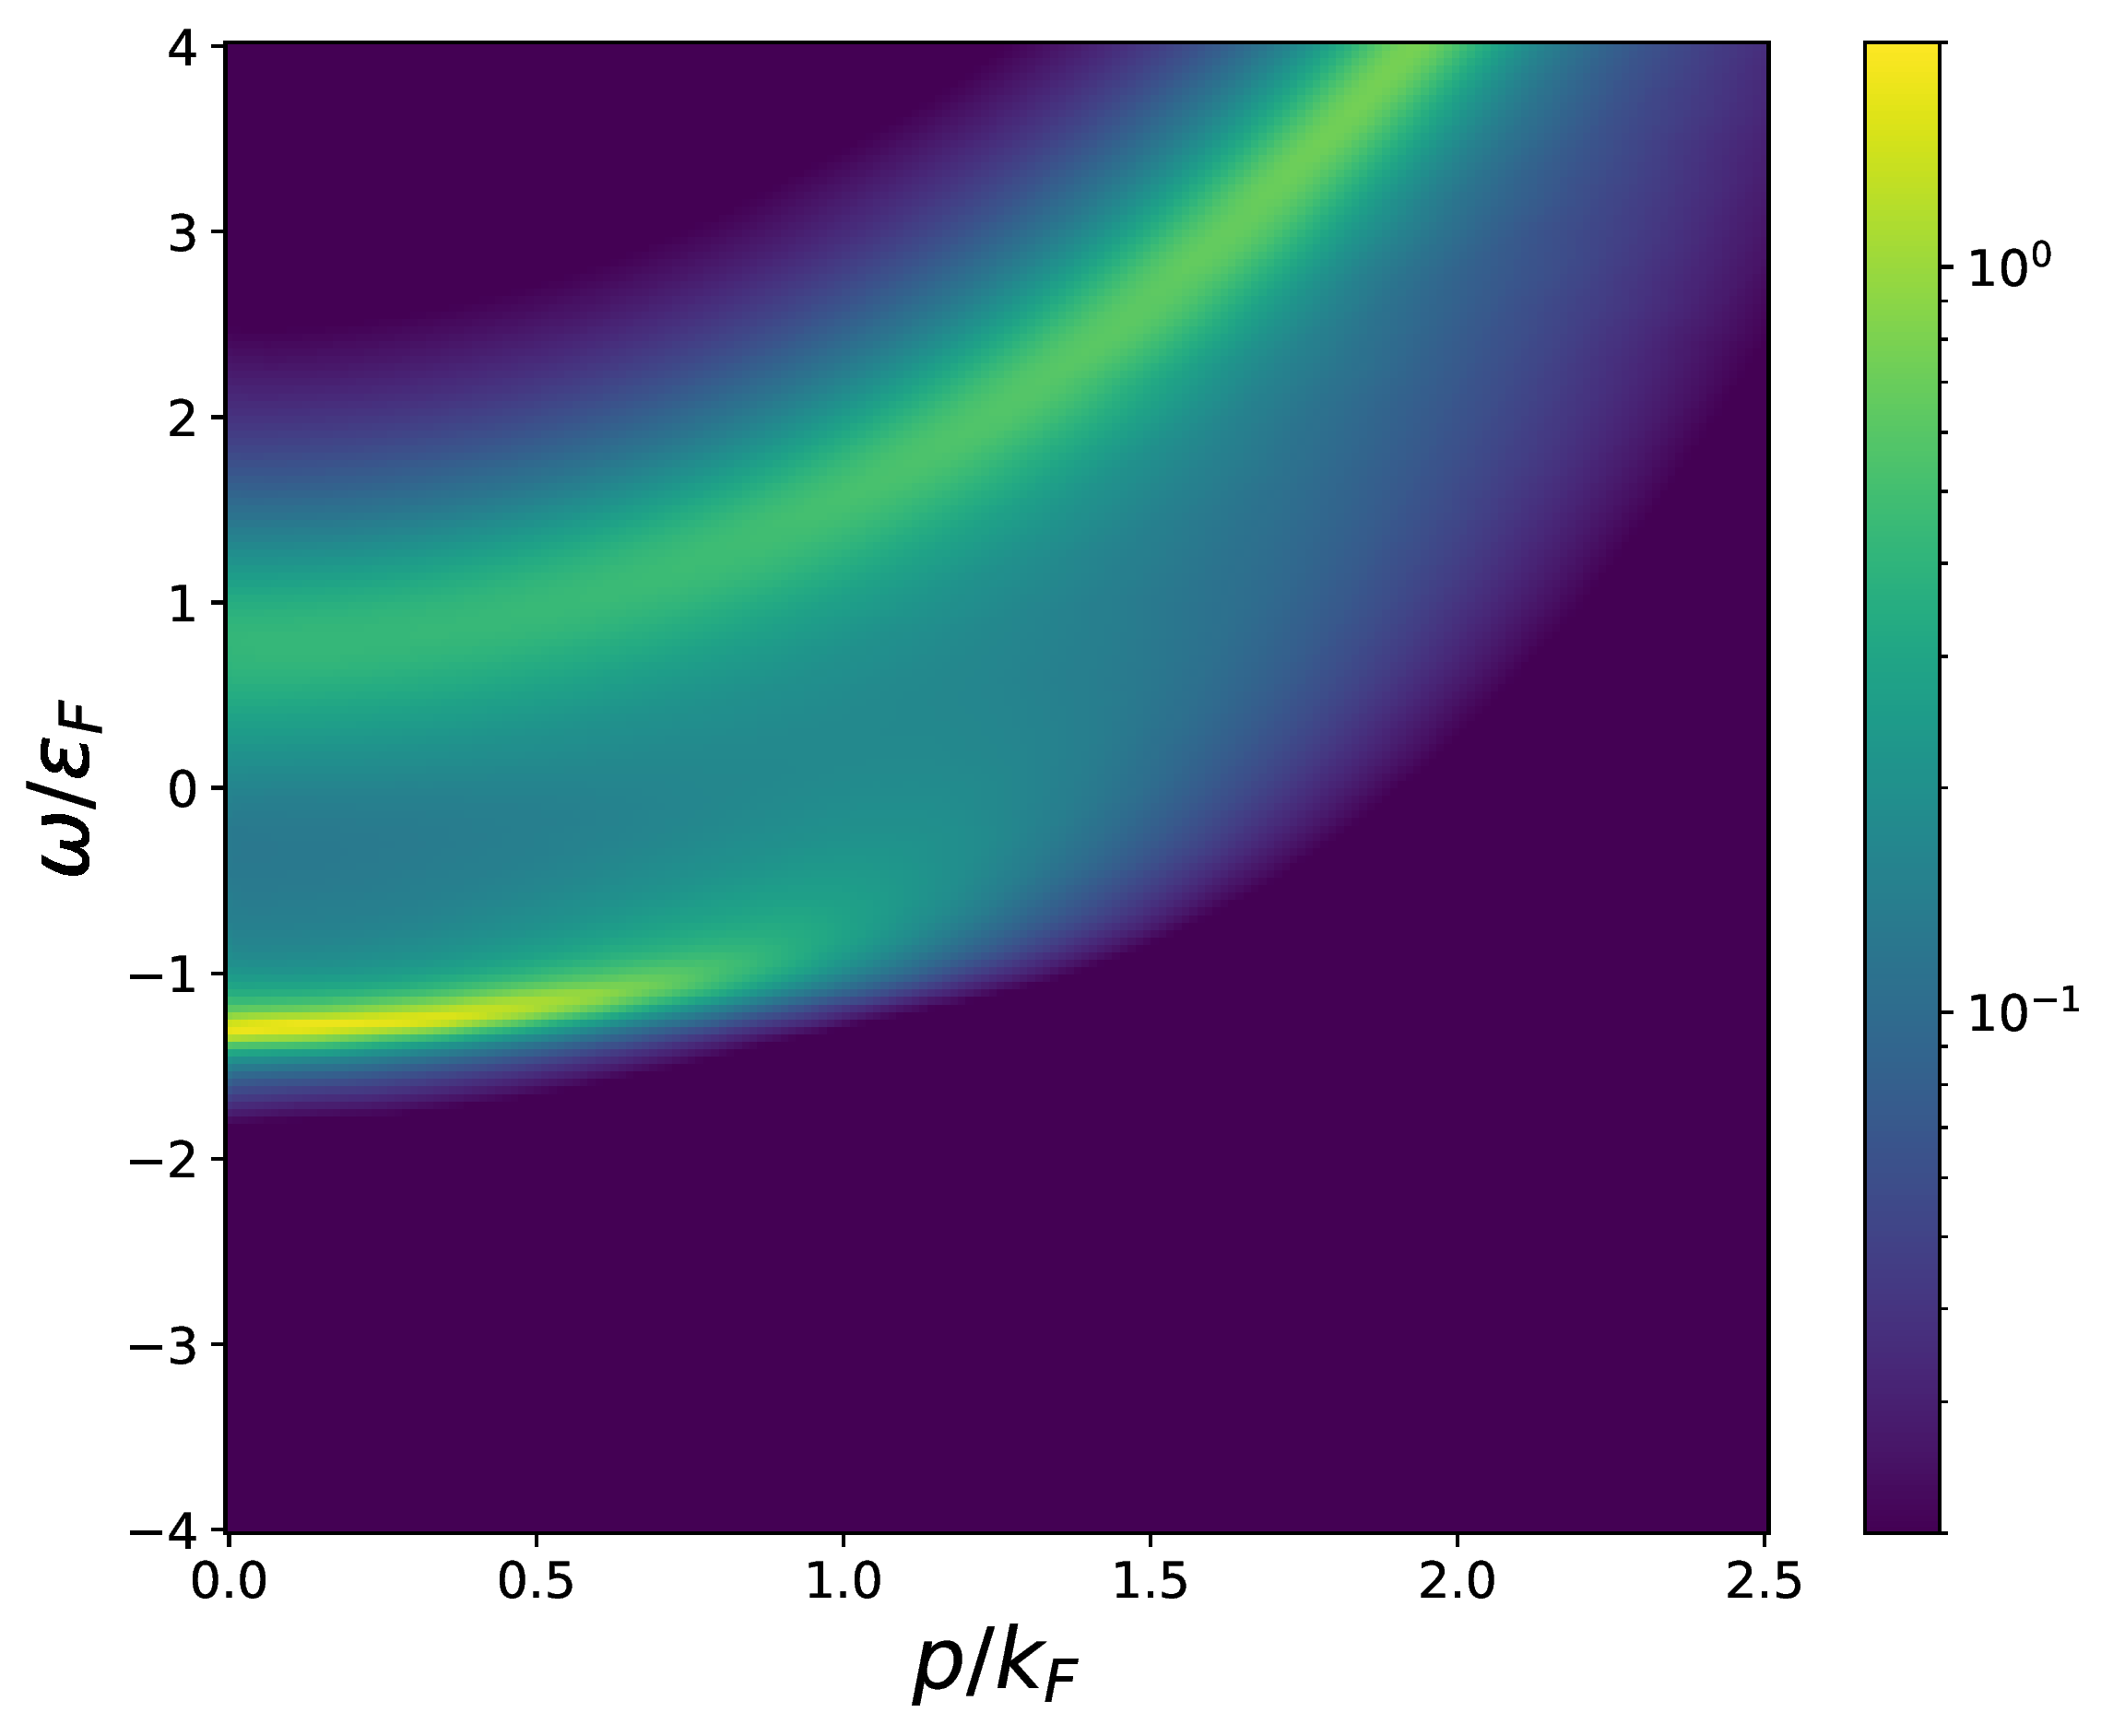
\includegraphics[width=0.24\textwidth]{figs/polaron_05kfa.png}}
	\subfigure[$(k_Fa)^{-1} = 1$]{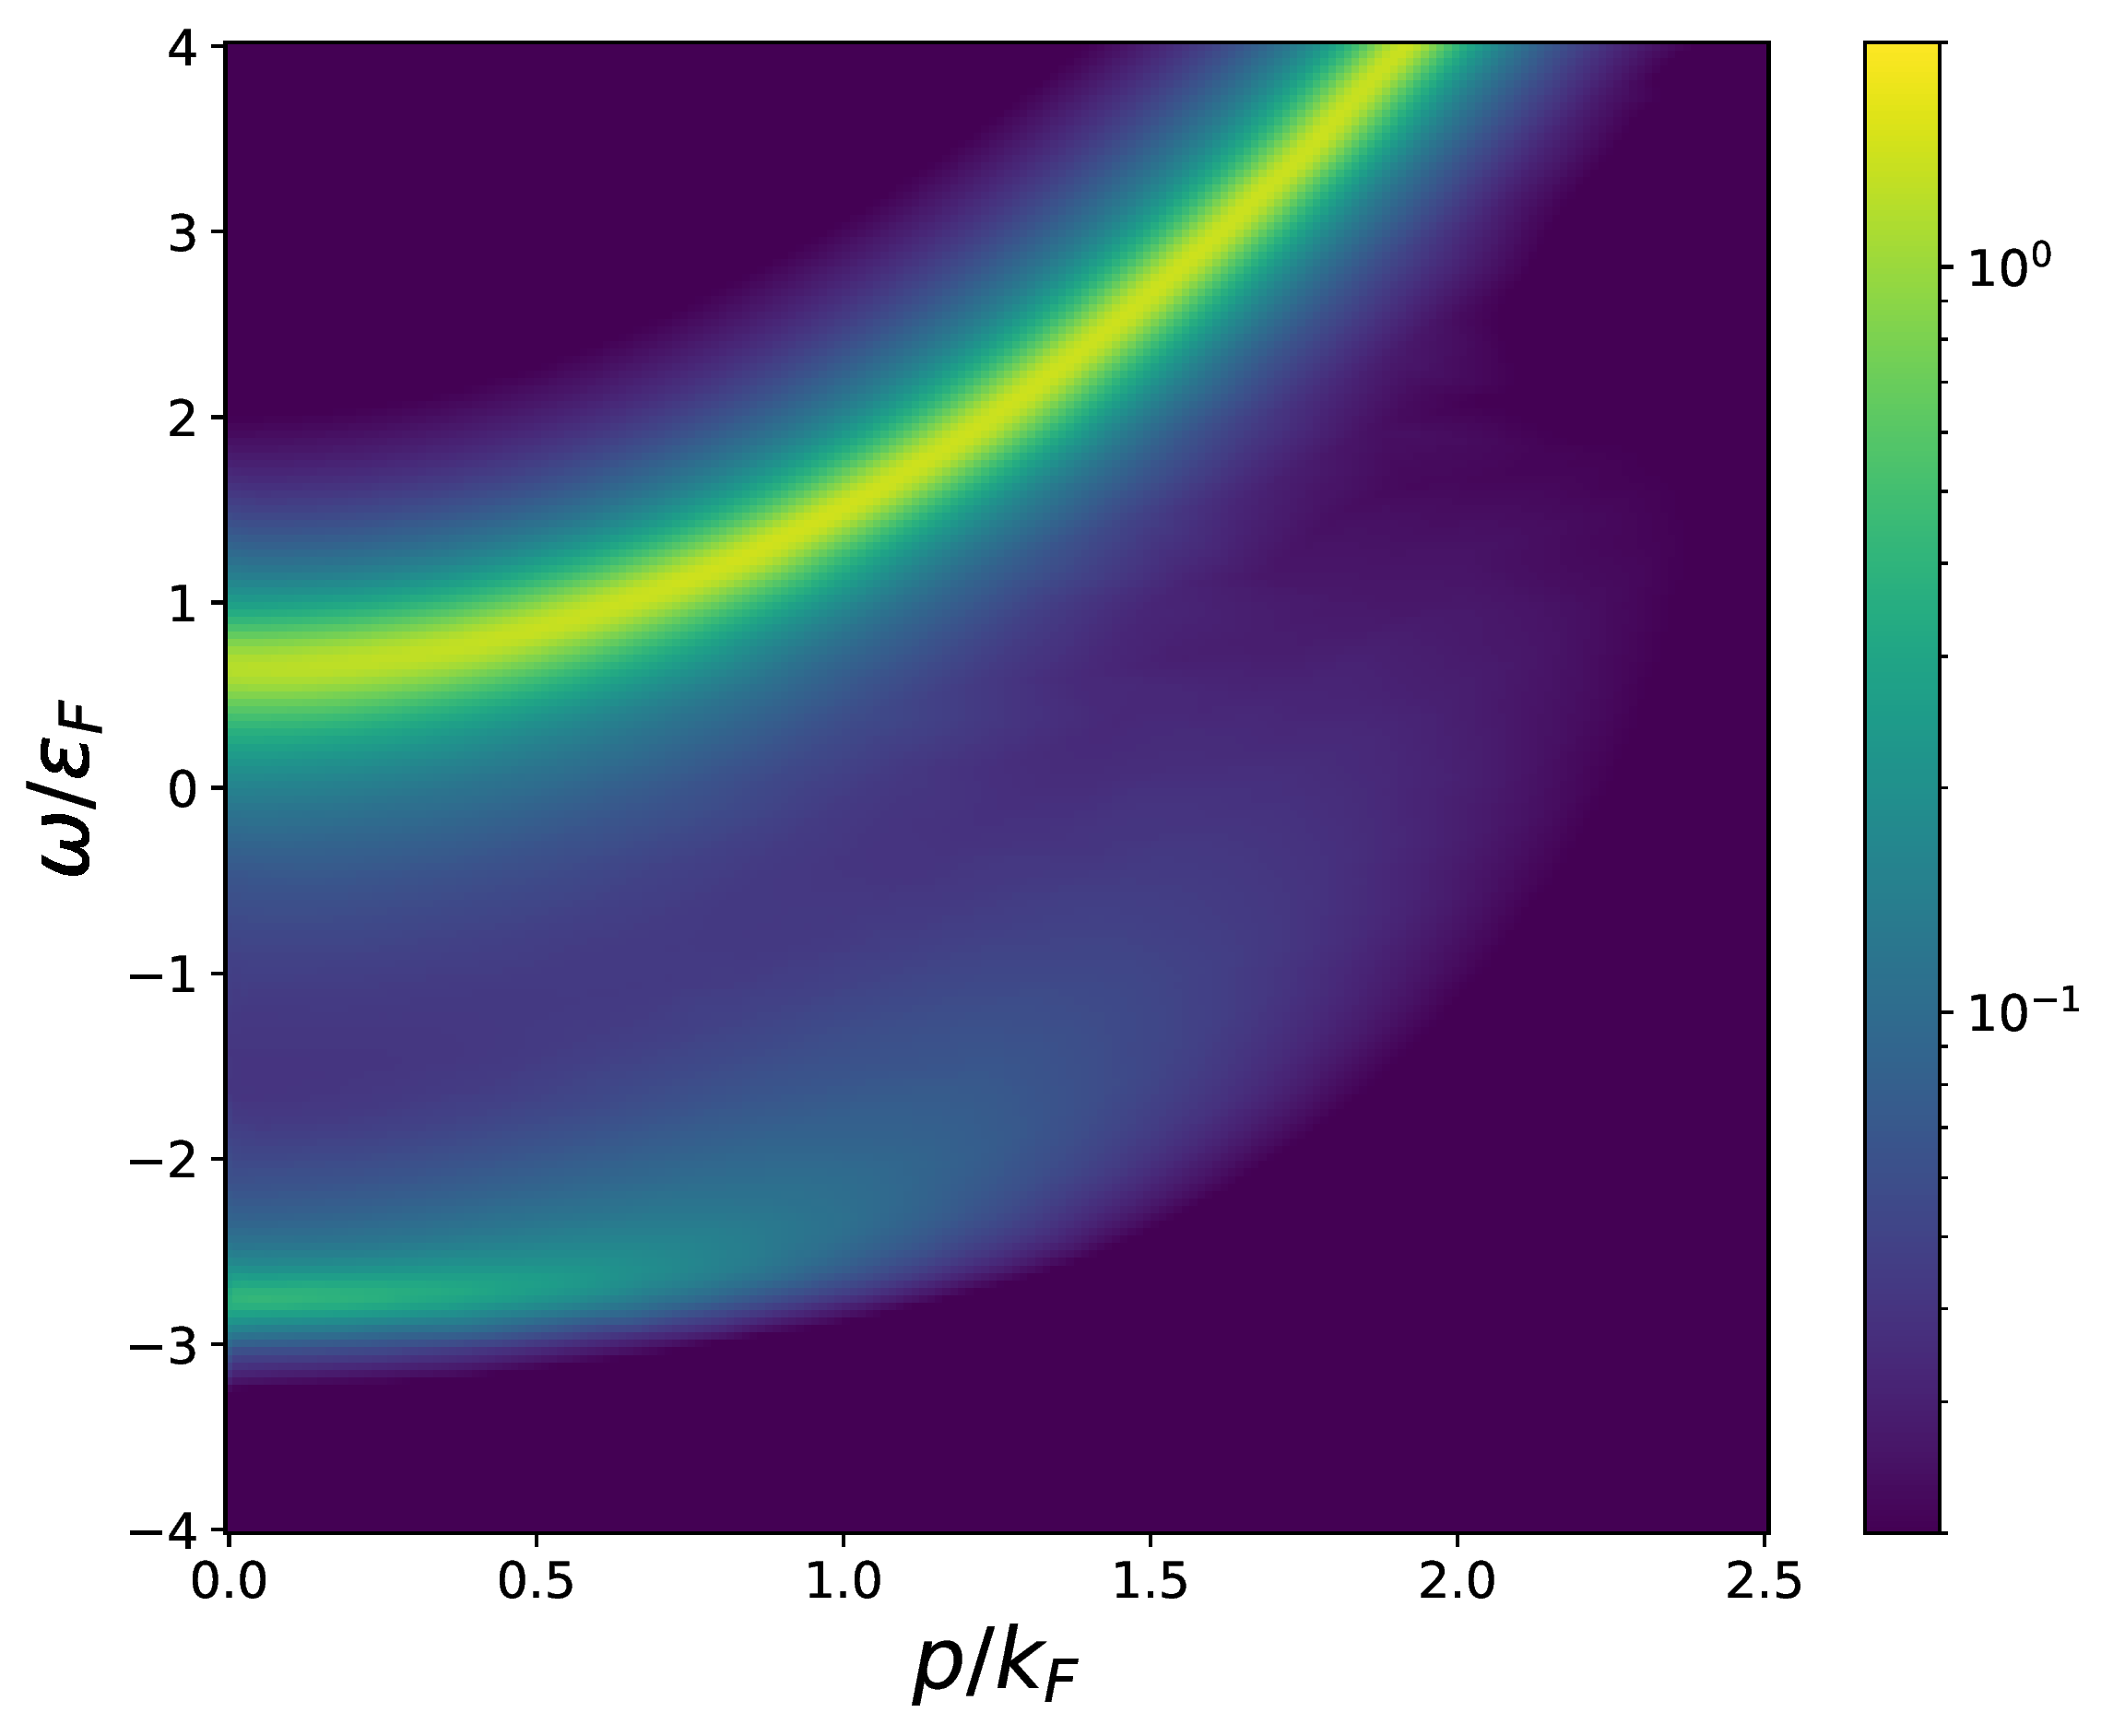
\includegraphics[width=0.24\textwidth]{figs/polaron_1kfa.png}}
	\caption[Spectral functions of Fermi polaron at different interaction strengths]{Results for the Fermi polaron spectral function $\rho_{\downarrow}\,\varepsilon_F$ at $T=0$ at different interaction strengths $(k_Fa)^{-1}$. These results agree well with~\cite{Schmidt2011,Kamikado2017}.}
	\label{fig:specs-comparison}
\end{figure}

From the spectral functions one can obtain important information about the physics of the system. First of all, one can notice the appearance of a second peak for larger interaction strengths $(k_Fa)^{-1}$ while the first one disappears. This is known as the repulsive polaron~\cite{Scazza2022}. Furthermore, one can notice the shift in ground state energy and a changing slope of the attractive polaron peak. Together with the boson ground state energy, the first observation leads to the well-known polaron-to-molecule transition~\cite{Schmidt2011}. The second observation is connected to the divergent effective mass of the attractive polaron~\cite{Vlietinck2013}. For larger interaction strengths the slope gets smaller, which corresponds to a larger effective mass. Eventually, the slope gets zero and can bend back. Besides the effective mass, other quasiparticle properties like the weight $Z$, decay width $\Gamma$ or the contact $C$ can be computed from the spectral function~\cite{Scazza2022}.

Fig.~\ref{fig:effect-finite-temperature} shows the effect of finite temperature in the Fermi polaron problem. One can see that the quasiparticle peak at low momenta gets broadened significantly and slightly shifted. Away from unitarity, one can also observe other phenomena, see~\cite{Hu2022} for more details. Note that the chemical potential $\mu_{\uparrow}(T)$ of the majority particles is temperature-dependent and has to be determined from the number equation for an ideal Fermi gas, see Section~\ref{section:results}. At $T=0.2\,T_F$, the chemical potential is $\mu_{\uparrow}=0.964$. It is compelling to investigate quasiparticle properties as a function of $T$, some of which are considered in~\cite{Hu2022}. One could, for example, compute the quasiparticle weight $Z(T)$ or the contact $C(T)$. It is anticipated that $Z$ should tend to unity for large temperatures, as the spectral function becomes more and more classical. Unfortunately, this analysis could not be finalized before the submission of this Thesis.

In Fig.~\ref{fig:impurity-convergence}, the convergence behavior of the polaron spectral function for two different temperatures is shown. Similar to the spin-balanced BCS-BEC case in Section~\ref{section:results}, the spectral function at higher temperature converges faster and smoother. However, only 5-6 iterations are needed to converge in the polaron case. This is again due to the fact that the majority particles are not dressed and strong correlations do not play a significant role. It is observed that the change from the first to the second iteration is very pronounced, however, further iterations have not so much impact. Other comparisons of non-selfconsistent and selfconsistent results can be found in~\cite{Chien2010,Hu2008,Tajima2021}. In the following, we will make this comparison more explicit by using calculated ejection rf spectra.

Recently, rf spectra and contact of an extremely spin-imbalanced Fermi gas at unitarity were measured at MIT~\cite{Yan2019}. Shortly after, Tajima et al. published first considerations in~\cite{Tajima2019}, and last year Hu et al. published non-selfconsistent real-time results in~\cite{Hu2022}. Here, we want to extend these results to selfconsistent rf spectra.

\begin{figure}[h]
	\centering
	\subfigure[$T=0$]{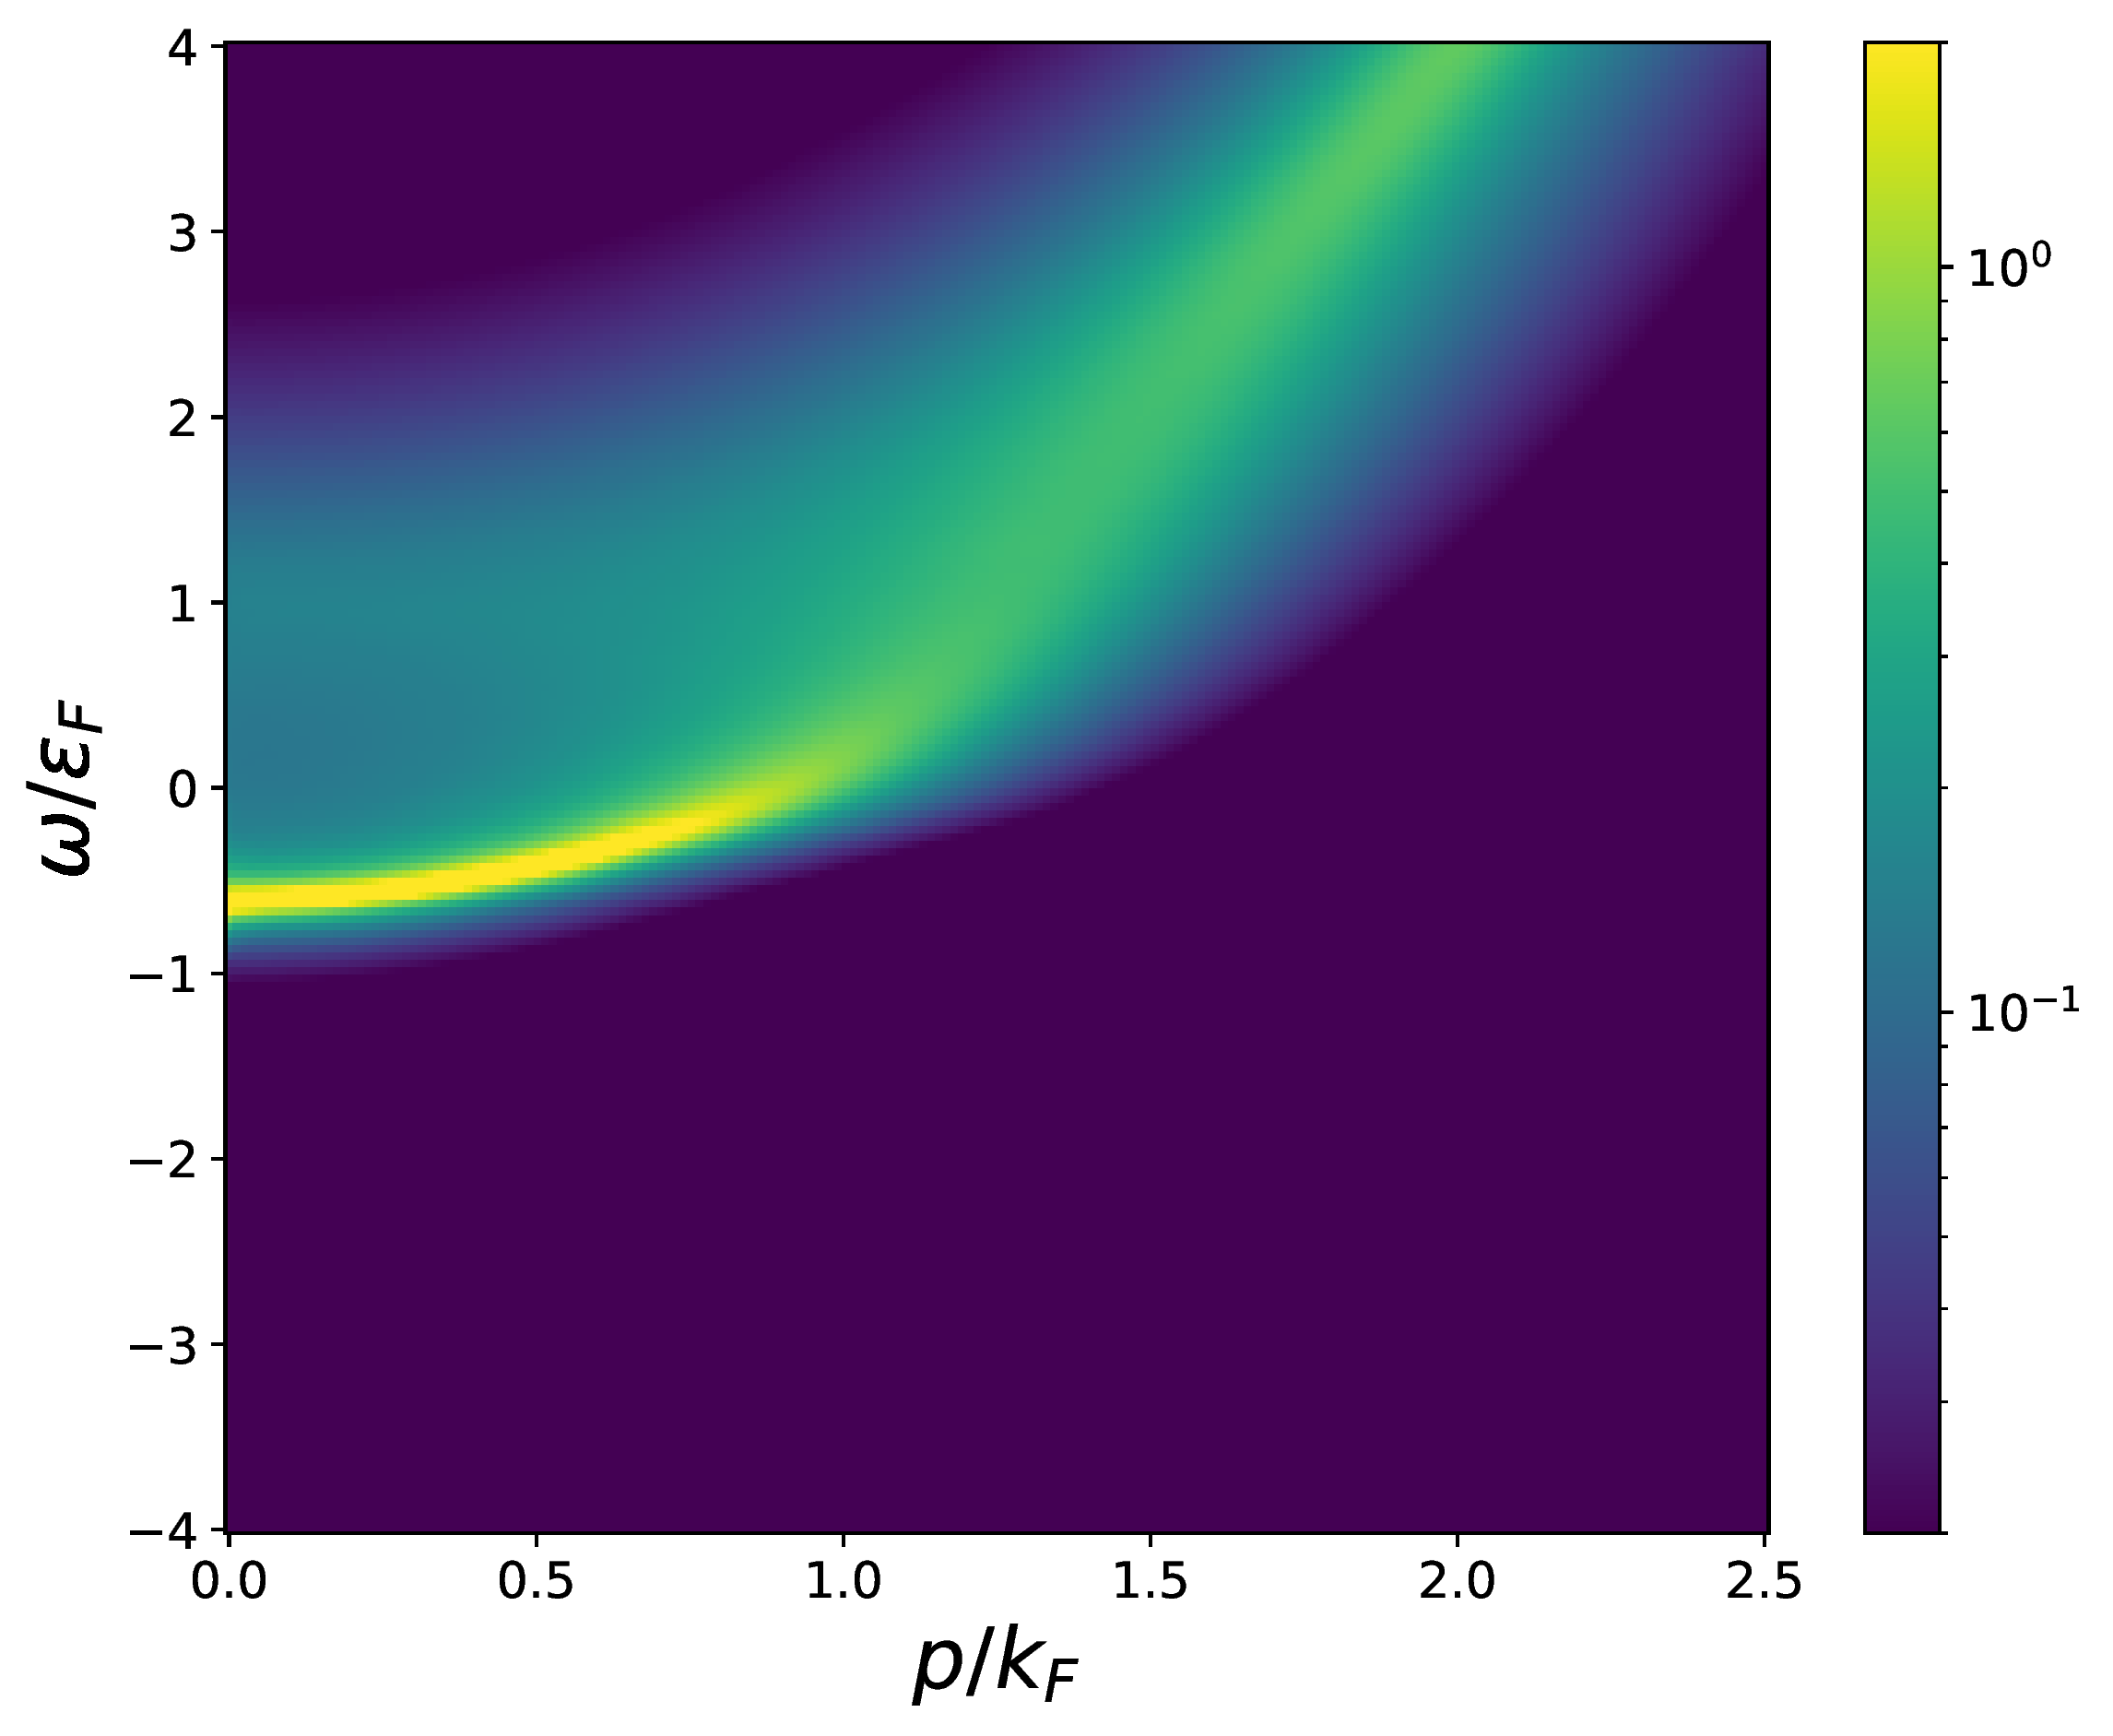
\includegraphics[width=0.468\textwidth]{figs/polaron_unitary0.png}} 
	\subfigure[$T=0.2T_F$]{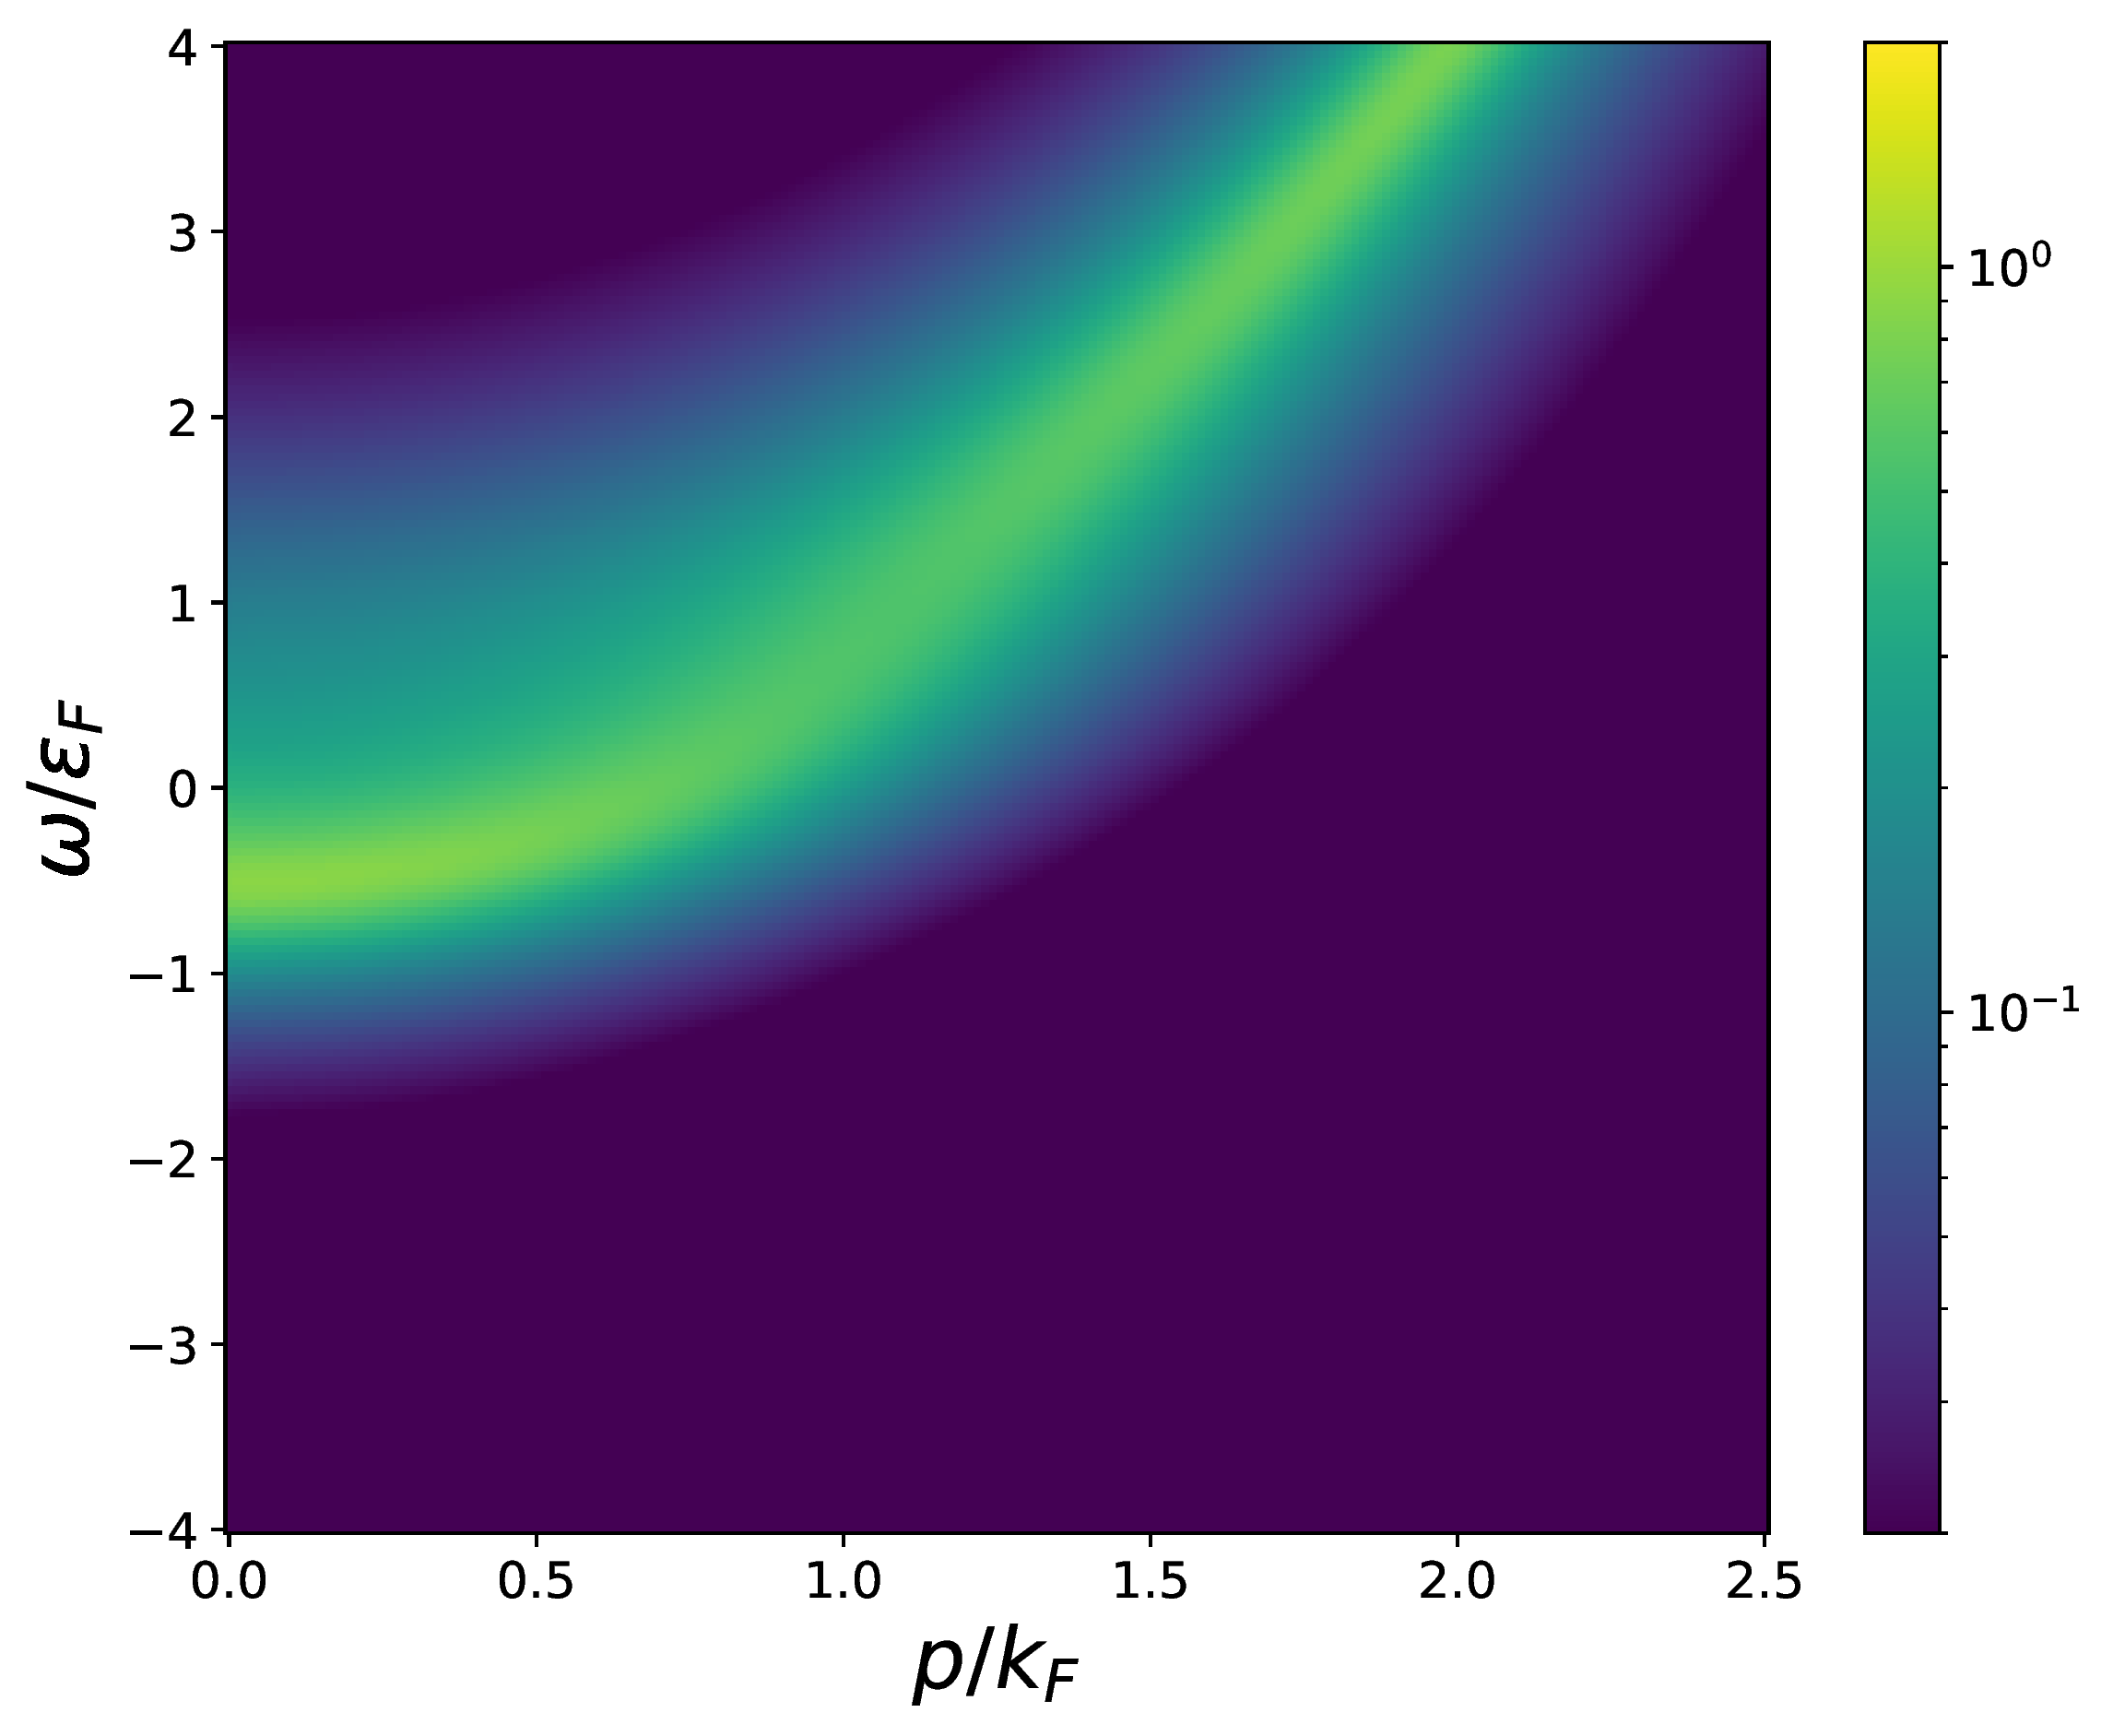
\includegraphics[width=0.468\textwidth]{figs/polaron_unitary02.png}} 
	\caption[Effect of finite temperature]{Effect of finite temperature. Spectral functions of the unitary Fermi polaron at (a) $T=0$ and (b) $T=0.2T_F$.}
	\label{fig:effect-finite-temperature}
\end{figure}

\newpage

\begin{figure}[h]
	\centering
	\subfigure[$T=0.2\,T_F$]{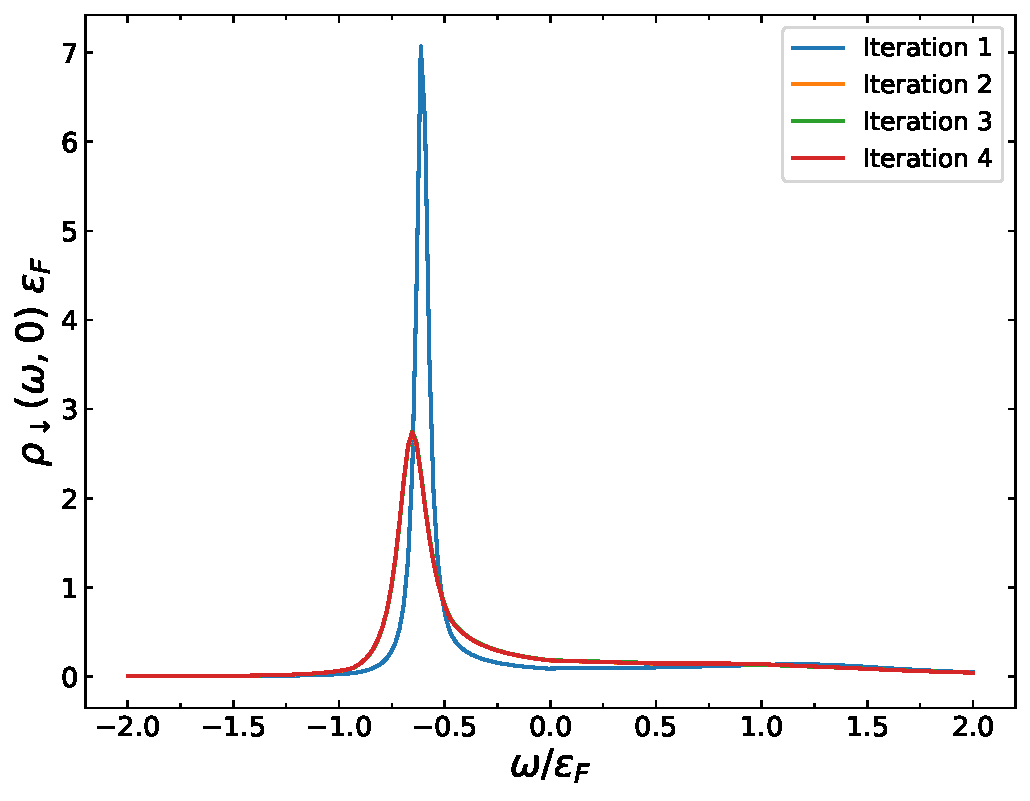
\includegraphics[width=0.468\textwidth]{figs/polaron_unitary02_convergence.pdf}}
	\subfigure[$T=0.8\,T_F$]{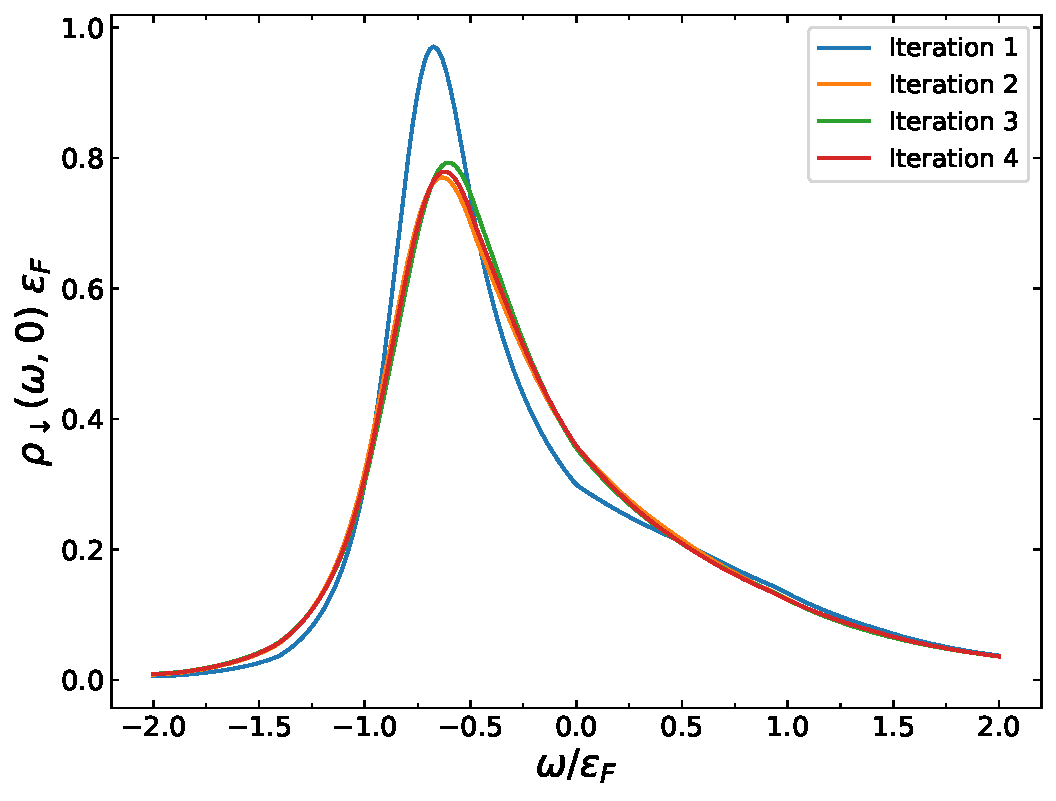
\includegraphics[width=0.476\textwidth]{figs/polaron_unitary08_convergence.pdf}}
	\caption[Convergence of polaron spectral function at different temperatures]{Convergence of the polaron spectral function at different temperatures.}
	\label{fig:impurity-convergence}
\end{figure}

Fig.~\ref{fig:rf-spectra-polaron} shows the non-selfconsistent and selfconsistent results for the polaron rf spectra. These results were obtained in the limit of zero impurity concentration using the same formula~\eqref{eq:rf-spectra} as in Section~\ref{section:results}, see also~\cite{Hu2022,Tajima2019}. For the polaron it reads
%
\begin{align}
	\label{eq:rf-spectra-polaron}
	I(\omega) = \int_{\bm{q}} \rho_{\downarrow}(\varepsilon^{(I)}_{\bm{q}}-\omega-\mu_{\downarrow},\bm{q})\, n_F(\varepsilon^{(I)}_{\bm{q}}-\omega-\mu_{\downarrow}) \,.
\end{align}
%
As mentioned above, we consider the mass-balanced case. The chemical potential of the impurity is $\mu_{\downarrow}=0$. As in the previous Section, the chemical potential of the Fermi sea $\mu_{\uparrow}(T)$ is temperature-dependent and has to be determined from the number equation. Additionally, a Fourier broadening of $0.1\varepsilon_F$ and a right-shift of $0.09\varepsilon_F$ were performed to account for the experimental features. It is found that these results agree well with previous work~\cite{Hu2022,Tajima2019}. However, both approaches cannot describe the experimental data in~\cite{Yan2019} correctly. Since the experimental setup was similar to~\cite{Mukherjee2019}, as discussed in Section~\ref{section:results} for the spin-balanced Fermi gas, the reason for this mismatch might be again the missing trap average for the harmonic trap potential. Other reasons for the mismatch are discussed in~\cite{Hu2022,Tajima2019} and could be due to absent many-body correlations which are not included in the T-matrix approach.

As an outlook for future work, the next step could be to investigate missing three-body correlations~\cite{Bruun2010,Tajima2019}. There exist some approaches to include those effects, however, fully selfconsistent real-time computations are lacking. The spectral method presented in this work provides excellent possibilities to incorporate such three-body diagrams while keeping computational costs quite reasonable. Another possibility would be to include momentum-dependent vertices, as discussed in~\cite{Diehl2006-1, Floerchinger2008, Falco2007, Romans2005, Romans2006}. This was already implemented successfully in the spectral functional approach for scalar field theory~\cite{Horak2020}.


\begin{figure}[htb]
	\begin{minipage}[t]{.492\textwidth}
		\centering
		\subfigure[]{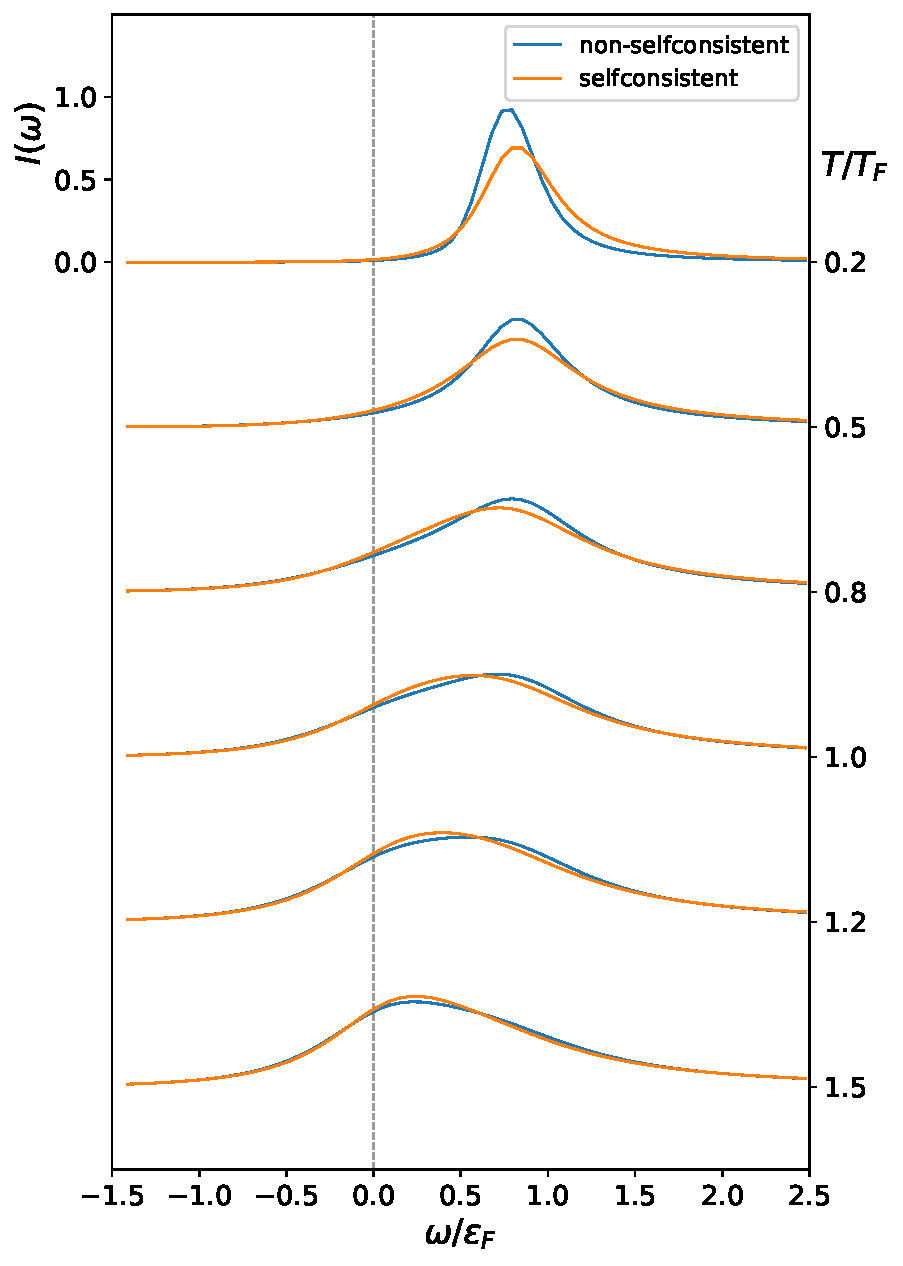
\includegraphics[width=\textwidth]{figs/rf_spectra_polaron.pdf}}
	\end{minipage}
	\hfill
	\begin{minipage}[t]{.49\textwidth}
		\centering
		\subfigure[]{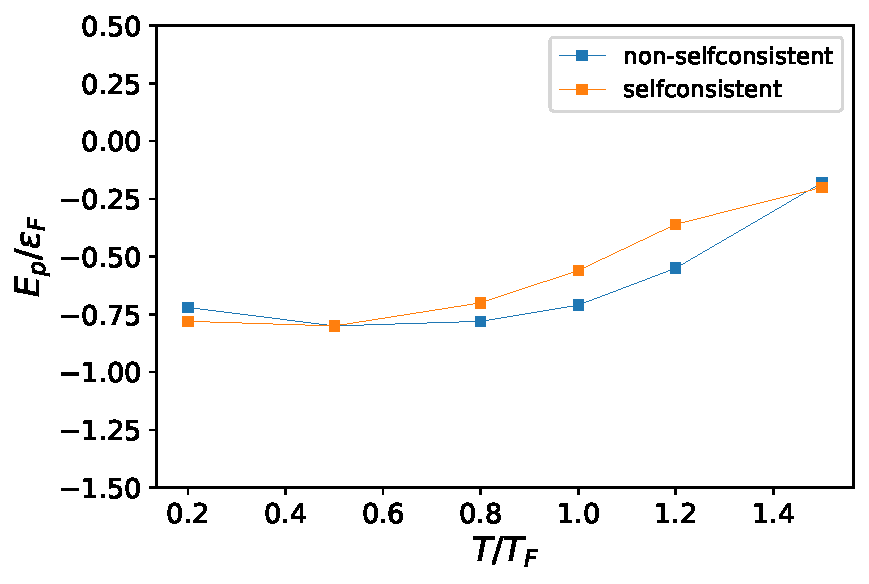
\includegraphics[width=0.95\textwidth]{figs/peakPositions.pdf}}
		\raggedleft
		\subfigure[]{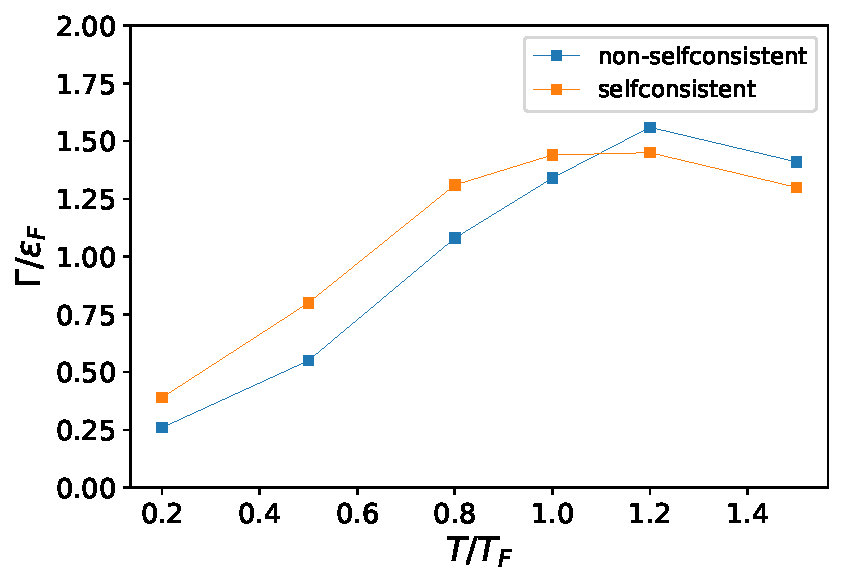
\includegraphics[width=0.92\textwidth]{figs/FWHM.pdf}}
	\end{minipage}
	\caption[Rf spectra of the unitary Fermi polaron]{(a) Calculated ejection rf spectra $I(\omega)$ for the unitary Fermi polaron as a function of the reduced temperature $T/T_F$. Non-selfconsistent results (blue solid lines) are compared to selfconsistent results (orange solid lines). A Fourier broadening of $0.1\varepsilon_F$ to account for the finite experimental resolution, and a right-shift by $0.09\varepsilon_F$ to account for the final state interaction were applied. (b) Peak position ($E_p=-\hbar\omega$) and (c) full width at half maximum $\Gamma$ extracted from the rf spectra.}
	\label{fig:rf-spectra-polaron}
\end{figure}